\documentclass[11pt, oneside]{article}   	% use "amsart" instead of "article" for AMSLaTeX format
\usepackage{geometry}                		% See geometry.pdf to learn the layout options. There are lots.
\geometry{letterpaper}                   		% ... or a4paper or a5paper or ... 
%\geometry{landscape}                		% Activate for rotated page geometry
\usepackage[parfill]{parskip}    		% Activate to begin paragraphs with an empty line rather than an indent
\usepackage{graphicx}				% Use pdf, png, jpg, or eps§ with pdflatex; use eps in DVI mode
								% TeX will automatically convert eps --> pdf in pdflatex		
								
\usepackage{listings}				% Source code
\usepackage{amssymb}
\usepackage{cite}
\usepackage{hyperref}				% Hyperlinks
\usepackage[nottoc,numbib]{tocbibind}	% 'References' in TOC

\graphicspath{{img/}}					% Relative path where the images are stored. 

\title{Instructions for \\ Web Audio Evaluation Tool}
\author{Nicholas Jillings, Brecht De Man and David Moffat}
\date{7 December 2015}							% Activate to display a given date or no date

\begin{document}
\maketitle

These instructions are about use of the Web Audio Evaluation Tool \cite{waet} on Windows and Mac OS X platforms. 
% TO DO: Linux

\tableofcontents

\clearpage

\section{Installation}
	Download the folder (\url{https://code.soundsoftware.ac.uk/hg/webaudioevaluationtool/archive/tip.zip}) and unzip in a location of your choice. 
	
	\subsection{Contents}
		The folder should contain the following elements: \\
		
		\textbf{Main folder:} 
			\begin{itemize}
	            	\item \texttt{analyse.html}: analysis and diagnostics of a set of result XML files
	            	\item \texttt{ape.css, core.css, graphics.css, mushra.css, structure.css}: style files (edit to change appearance)
	            	\item \texttt{ape.js}: JavaScript file for APE-style interface \cite{ape}
	            	\item \texttt{mushra.js}: JavaScript file for MUSHRA-style interface \cite{mushra}
	            	\item \texttt{CITING.txt, LICENSE.txt, README.txt}: text files with, respectively, the citation which we ask to include in any work where this tool or any portion thereof is used, modified or otherwise; the license under which the software is shared; and a general readme file.
	            	\item \texttt{core.js}: JavaScript file with core functionality
	            	\item \texttt{index.html}: webpage where interface should appear (includes link to test configuration XML)
	            	\item \texttt{jquery-2.1.4.js}: jQuery JavaScript Library
	            	\item \texttt{pythonServer.py}: webserver for running tests locally
	            	\item \texttt{pythonServer-legacy.py}: webserver with limited functionality (no automatic storing of output XML files)
	            	\item \texttt{save.php}: PHP script to store result XML files to web server\\
			\end{itemize}
	     \textbf{Documentation (./docs/)}
	         \begin{itemize}
	         		\item Instructions: PDF and \LaTeX source of these instructions
	            	\item Project Specification Document (\LaTeX/PDF)
	            	\item Results Specification Document (\LaTeX/PDF)
	            	\item SMC15: PDF and \LaTeX  source of corresponding SMC2015 publication \cite{waet}
	            	\item WAC2016: PDF and \LaTeX  source of corresponding WAC2016 publication\\
			\end{itemize}
         \textbf{Example project (./example\_eval/)}
            	\begin{itemize}
            		\item An example of what the set up XML should look like, with example audio files 0.wav-10.wav which are short recordings at 44.1kHz, 16bit of a woman saying the corresponding number (useful for testing randomisation and general familiarisation with the interface).\\ 
            	\end{itemize}
          \textbf{Output files (./saves/)}
            	\begin{itemize}
            		\item The output XML files of tests will be stored here by default by the \texttt{pythonServer.py} script.\\ 
            	\end{itemize}
          \textbf{Auxiliary scripts (./scripts/)}
            	\begin{itemize}
            		\item Helpful Python scripts for extraction and visualisation of data.\\ 
            	\end{itemize}
          \textbf{Test creation tool (./test\_create/)}
            	\begin{itemize}
            		\item Webpage for easily setting up your own test without having to delve into the XML.\\ 
            	\end{itemize}
                    	
	\subsection{Browser}
		As Microsoft Internet Explorer doesn't support the Web Audio API\footnote{\url{http://caniuse.com/\#feat=audio-api}}, you will need another browser like Google Chrome, Safari or Firefox (all three are tested and confirmed to work). 
		
		The tool is platform-independent and works in any browser that supports the Web Audio API. It does not require any specific, proprietary software. However, in case the tool is hosted locally (i.e. you are not hosting it on an actual webserver) you will need Python (2.7), which is a free programming language - see the next paragraph. 
	

\clearpage

\section{Test setup}

	\subsection{Sample rate}
		Depending on how the experiment is set up, audio is resampled automatically (the Web Audio default) or the sample rate is enforced. In the latter case, you will need to make sure that the sample rate of the system is equal to the sample rate of these audio files. For this reason, all audio files in the experiment will have to have the same sample rate. 

		Always make sure that all other digital equipment in the playback chain (clock, audio interface, digital-to-analog converter, ...) is set to this same sample rate.

		Note that upon changing the sampling rate, the browser will have to be restarted for the change to take effect. 
		
		\subsubsection{Mac OS X}
			To change the sample rate in Mac OS X, go to \textbf{Applications/Utilities/Audio MIDI Setup} or find this application with Spotlight (see Figure \ref{fig:audiomidisetup}). Then select the output of the audio interface you are using and change the `Format' to the appropriate number. Also make sure the bit depth and channel count are as desired. 
			If you are using an external audio interface, you may have to go to the preference pane of that device to change the sample rate. 

			Also make sure left and right channel gains are equal, as some applications alter this without changing it back, leading to a predominantly louder left or right channel. See Figure \ref{fig:audiomidisetup} for an example where the channel gains are different. 

			\begin{figure}[tb]
				\centering
				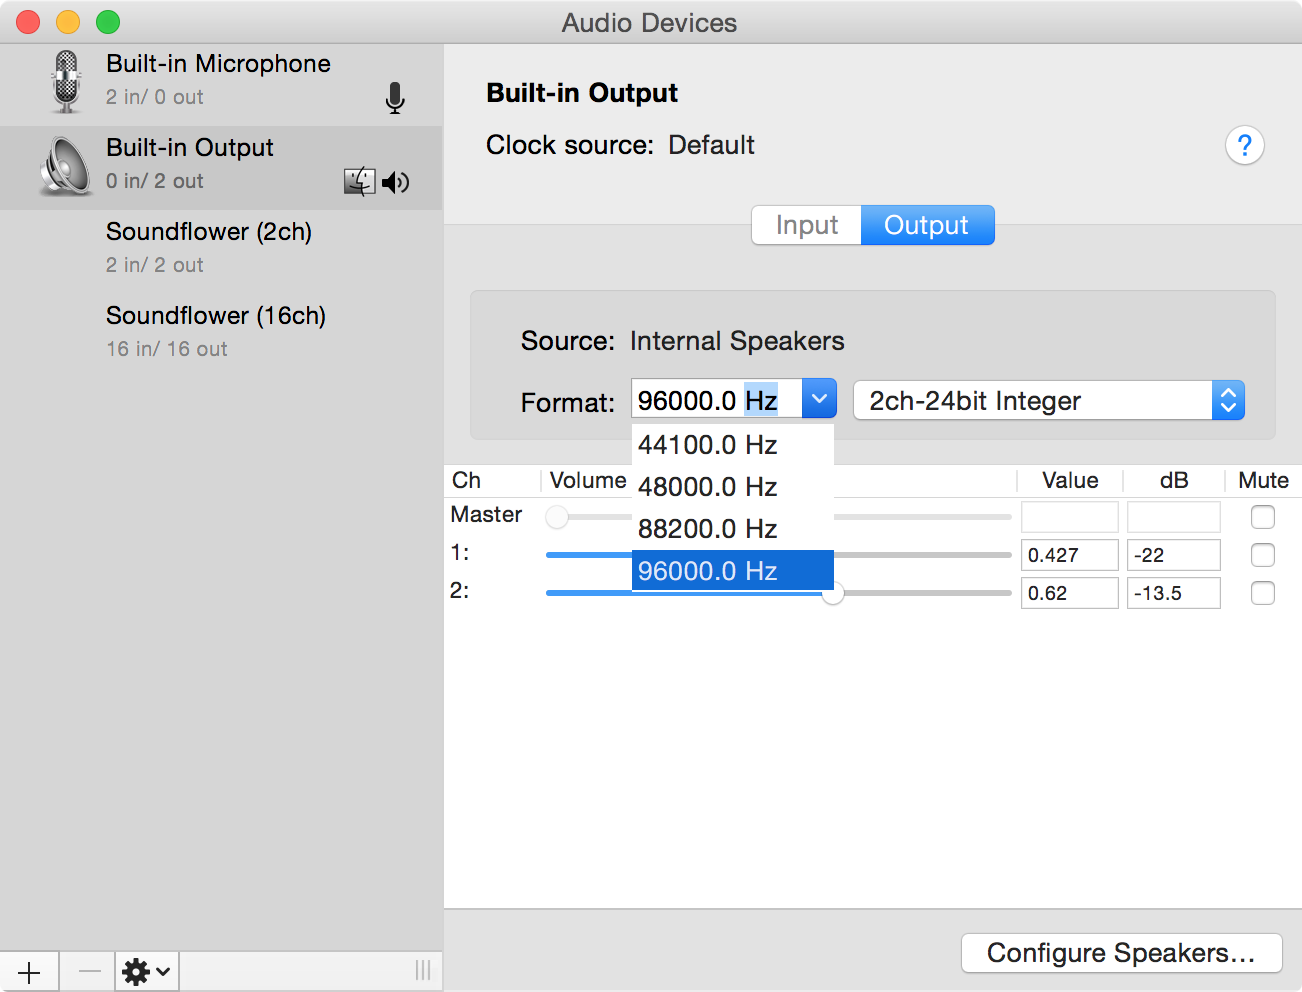
\includegraphics[width=.65\textwidth]{img/audiomidisetup.png}
				\caption{The Audio MIDI Setup window in Mac OS X}
				\label{fig:audiomidisetup}
			\end{figure}
		
		\subsubsection{Windows}
			To change the sample rate in Windows, right-click on the speaker icon in the lower-right corner of your desktop and choose `Playback devices'. Right-click the appropriate playback device and click `Properties'. Click the `Advanced' tab and verify or change the sample rate under `Default Format'.    % NEEDS CONFIRMATION
			If you are using an external audio interface, you may have to go to the preference pane of that device to change the sample rate. 

	\subsection{Local test}
		If the test is hosted locally, you will need to run the local webserver provided with this tool. 
		
		\subsubsection{Mac OS X}

			On Mac OS X, Python comes preinstalled. 

			Open the Terminal (find it in \textbf{Applications/Terminal} or via Spotlight), and go to the folder you downloaded. To do this, type \texttt{cd [folder]}, where \texttt{[folder]} is the folder where to find the \texttt{pythonServer.py} script you downloaded. For instance, if the location is \texttt{/Users/John/Documents/test/}, then type
			
				\texttt{cd /Users/John/Documents/test/}
				
			Then hit enter and run the Python script by typing

				\texttt{python pythonServer.py}

			and hit enter again. See also Figure \ref{fig:terminal}.
			
			\begin{figure}[htbp]
	                \begin{center}
	                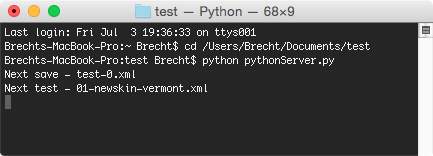
\includegraphics[width=.75\textwidth]{pythonServer.png}
	                \caption{Mac OS X: The Terminal window after going to the right folder (\texttt{cd [folder\_path]}) and running \texttt{pythonServer.py}.}
	                \label{fig:terminal}
	                \end{center}
	                \end{figure}

	        Alternatively, you can simply type \texttt{python} (follwed by a space) and drag the file into the Terminal window from Finder. % DOESN'T WORK YET
			
			You can leave this running throughout the different experiments (i.e. leave the Terminal open). 

			To start the test, open the browser and type 
				
			\texttt{localhost:8000}

			and hit enter. The test should start (see Figure \ref{fig:test}). 

			To quit the server, either close the terminal window or press Ctrl+C on your keyboard to forcibly shut the server.

		\subsubsection{Windows}

			On Windows, Python 2.7 is not generally preinstalled and therefore has to be downloaded\footnote{\url{https://www.python.org/downloads/windows/}} and installed to be able to run scripts such as the local webserver, necessary if the tool is hosted locally. 
		
			Simply double click the Python script \texttt{pythonServer.py} in the folder you downloaded. 
			
			You may see a warning like the one in Figure \ref{fig:warning}. Click `Allow access'. 
			
			\begin{figure}[htbp]
            \begin{center}
            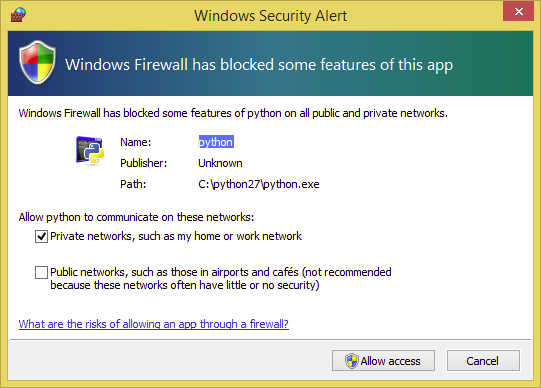
\includegraphics[width=.6\textwidth]{warning.png}
            \caption{Windows: Potential warning message when executing \texttt{pythonServer.py}.}
            \label{fig:warning}
            \end{center}
            \end{figure}
            
            The process should now start, in the Command prompt that opens - see Figure \ref{fig:python}. 
            
            \begin{figure}[htbp]
            \begin{center}
            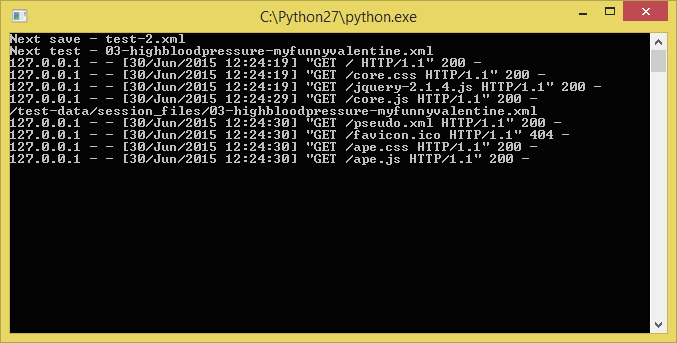
\includegraphics[width=.75\textwidth]{python.png}
            \caption{Windows: The Command Prompt after running \texttt{pythonServer.py} and opening the corresponding website.}
            \label{fig:python}
            \end{center}
            \end{figure}
            
            You can leave this running throughout the different experiments (i.e. leave the Command Prompt open). 

		    To start the test, open the browser and type 
				
			\texttt{localhost:8000}
		
			and hit enter. The test should start (see Figure \ref{fig:test}). 
		
			\begin{figure}[htb]
	        \begin{center}
	        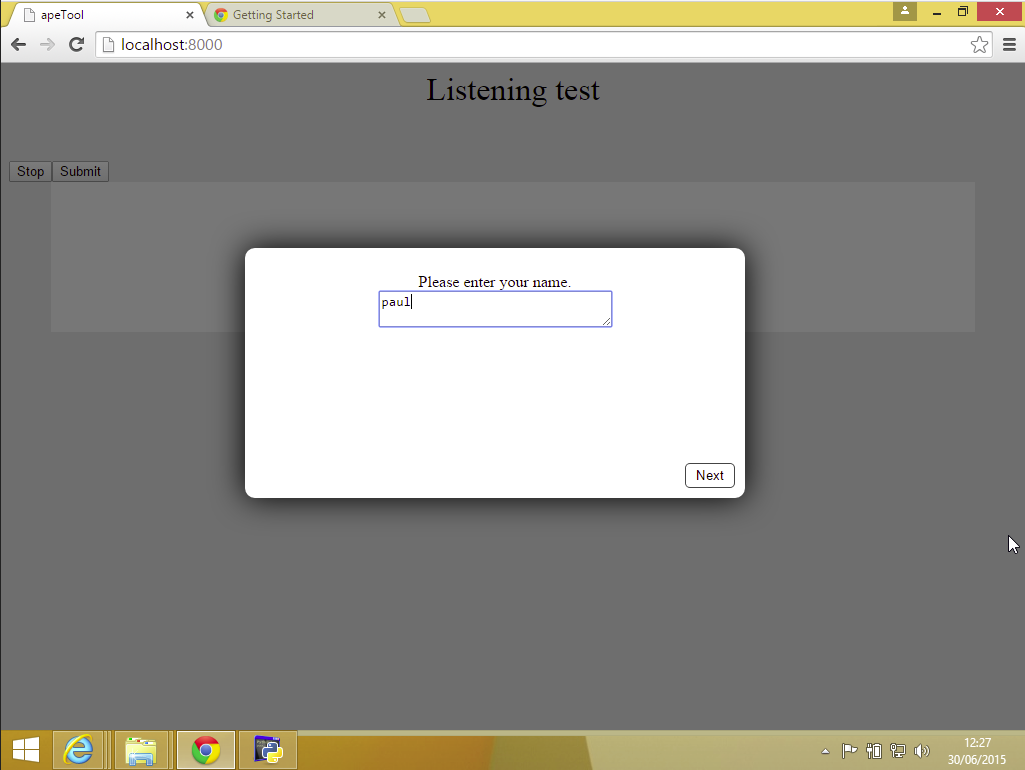
\includegraphics[width=.8\textwidth]{test.png}
	        \caption{The start of the test in Google Chrome on Windows 7.}
	        \label{fig:test}
	        \end{center}
	        \end{figure}
                    
        If at any point in the test the participant reports weird behaviour or an error of some kind, or the test needs to be interrupted, please notify the experimenter and/or refer to Section \ref{sec:troubleshooting}. 
		
		When the test is over (the subject should see a message to that effect, and click `Submit' one last time), the output XML file containing all collected data should have appeared in `saves/'. The names of these files are `test-0.xml', `test-1.xml', etc., in ascending order. The Terminal or Command prompt running the local web server will display the following file name. If such a file did not appear, please again refer to Section \ref{sec:troubleshooting}. 
		
		It is advised that you back up these results as often as possible, as a loss of this data means that the time and effort spent by the subject(s) has been in vain. Save the results to an external or network drive, and/or send them to the experimenter regularly. 
		
		To start the test again for a new participant, you do not need to close the browser or shut down the Terminal or Command Prompt. Simply refresh the page or go to \texttt{localhost:8000} again. 
		

	\subsection{Remote test}
		Put all files on a web server which supports PHP. This allows the `save.php' script to store the XML result files in the `saves/' folder. If the web server is not able to store the XML file there at the end of the test, it will present the XML file locally to the user, as a `Save file' link. 
		
\clearpage
	

\section{Using the test create tool}
	We provide a test creation tool, available in the directory test\_create. This tool is a self-contained web page, so doubling clicking will launch the page in your system default browser.

	The test creation tool can help you build a simple test very quickly. By simply selecting your interface and clicking check-boxes you can build a test in minutes.

	Include audio by dragging and dropping the stimuli you wish to include. 

	The tool examines your XML before exporting to ensure you do not export an invalid XML structure which would crash the test.
	
	This guide will help you to construct your own interface on top of the WAET (Web Audio Evaluation Tool) engine. The WAET engine resides in the core.js file, this contains prototype objects to handle most of the test creation, operation and data collection. The interface simply has to link into this at the correct points.

	\subsection{Nodes to familiarise}
		Core.js handles several very important nodes which you should become familiar with. The first is the Audio Engine, initialised and stored in variable `AudioEngineContext'. This handles the playback of the web audio nodes as well as storing the `AudioObjects'. The `AudioObjects' are custom nodes which hold the audio fragments for playback. These nodes also have a link to two interface objects, the comment box if enabled and the interface providing the ranking. On creation of an `AudioObject' the interface link will be nulled, it is up to the interface to link these correctly.

		The specification document will be decoded and parsed into an object called `specification'. This will hold all of the specifications various nodes. The test pages and any pre/post test objects are processed by a test state which will proceed through the test when called to by the interface. Any checks (such as playback or movement checks) are to be completed by the interface before instructing the test state to proceed. The test state will call the interface on each page load with the page specification node.

	\subsection{Modifying \texttt{core.js}}
		Whilst there is very little code actually needed, you do need to instruct core.js to load your interface file when called for from a specification node. There is a function called `loadProjectSpecCallback' which handles the decoding of the specification and setting any external items (such as metric collection). At the very end of this function there is an if statement, add to this list with your interface string to link to the source. There is an example in there for both the APE and MUSHRA tests already included. Note: Any updates to core.js in future work will most likely overwrite your changes to this file, so remember to check your interface is still here after any update that interferes with core.js.
		Any further files can be loaded here as well, such as css styling files. jQuery is already included.

	\subsection{Building the Interface}
		Your interface file will get loaded automatically when the `interface' attribute of the setup node matches the string in the `loadProjectSpecCallback' function. The following functions must be defined in your interface file.
		\begin{itemize}
		\item \texttt{loadInterface} - Called once when the document is parsed. This creates any necessary bindings, such as to the metric collection classes and any check commands. Here you can also start the structure for your test such as placing in any common nodes (such as the title and empty divs to drop content into later).
		\item \texttt{loadTest(audioHolderObject)} - Called for each page load. The audioHolderObject contains a specification node holding effectively one of the audioHolder nodes.
		\item \texttt{resizeWindow(event)} - Handle for any window resizing. Simply scale your interface accordingly. This function must be here, but can me an empty function call.
		\end{itemize}

		\subsubsection{loadInterface}
			This function is called by the interface once the document has been parsed since some browsers may parse files asynchronously. The best method is simply to put `loadInterface()' at the top of your interface file, therefore when the JavaScript engine is ready the function is called.

			By default the HTML file has an element with id ``topLevelBody'' where you can build your interface. Make sure you blank the contents of that object. This function is the perfect time to build any fixed items, such as the page title, session titles, interface buttons (Start, Stop, Submit) and any holding and structure elements for later on.

			At the end of the function, insert these two function calls: testState.initialise() and testState.advanceState();. This will actually begin the test sequence, including the pre-test options (if any are included in the specification document).

		\subsubsection{loadTest(audioHolderObject)}
			This function is called on each new test page. It is this functions job to clear out the previous test and set up the new page. Use the function audioEngineContext.newTestPage(); to instruct the audio engine to prepare for a new page. ``audioEngineContext.audioObjects = [];'' will delete any audioObjects, interfaceContext.deleteCommentBoxes(); will delete any comment boxes and interfaceContext.deleteCommentQuestions(); will delete any extra comment boxes specified by commentQuestion nodes.

			This function will need to instruct the audio engine to build each fragment. Just passing the constructor each element from the audioHolderObject will build the track, audioEngineContext.newTrack(element) (where element is the audioHolderObject audio element). This will return a reference to the constructed audioObject. Decoding of the audio will happen asynchronously.

			You also need to link audioObject.interfaceDOM with your interface object for that audioObject. The interfaceDOM object has a few default methods. Firstly it must start disabled and become enabled once the audioObject has decoded the audio (function call: enable()). Next it must have a function exportXMLDOM(), this will return the xml node for your interface, however the default is for it to return a value node, with textContent equal to the normalised value. You can perform other functions, but our scripts may not work if something different is specified (as it will breach our results specifications). Finally it must also have a method getValue, which returns the normalised value.

			It is also the job the interfaceDOM to call any metric collection functions necessary, however some functions may be better placed outside (for example, the APE interface uses drag and drop, therefore the best way was to call the metric functions from the dragEnd function, which is called when the interface object is dropped). Metrics based upon listening are handled by the audioObject. The interfaceDOM object must manage any movement metrics. For a list of valid metrics and their behaviours, look at the project specification document included in the repository/docs location. The same goes for any checks required when pressing the submit button, or any other method to proceed the test state.



\clearpage
\section{Troubleshooting} \label{sec:troubleshooting}
	Thanks to feedback from using the interface in experiments by the authors and others, many bugs have been caught and fatal crashes due to the interface (provided it is set up properly by the user) seem to be a thing of the past. 

	However, if things do go wrong or the test needs to be interrupted for whatever reason, all data is not lost. In a normal scenario, the test needs to be completed until the end (the final `Submit'), at which point the output XML is stored in the \texttt{saves/}. If this stage is not reached, open the JavaScript Console (see below for how to find it) and type 

	\texttt{createProjectSave()}

	to present the result XML file on the client side, or

	\texttt{createProjectSave(specification.projectReturn)}

	to try to store it to the specified location, e.g. the `saves/' folder on the web server or the local machine (on failure the result XML should be presented directly in the web browser instead)

	and hit enter. This will open a pop-up window with a hyperlink that reads `Save File'; click it and an XML file with results until that point should be stored in your download folder. 
	
	Alternatively, a lot of data can be read from the same console, in which the tool prints a lot of debug information. Specifically:
    	\begin{itemize}
        	\item the randomisation of pages and fragments are logged;
        	\item any time a slider is played, its ID and the time stamp (in seconds since the start of the test) are displayed;
        	\item any time a slider is dragged and dropped, the location where it is dropped including the time stamp are shown; 
        	\item any comments and pre- or post-test questions and their answers are logged as well. 
    	\end{itemize}

	You can select all this and save into a text file, so that none of this data is lost. You may to choose to do this even when a test was successful as an extra precaution. 

	If you encounter any issue which you believe to be caused by any aspect of the , or which the documentation does not mention, please do let us know! 

	\subsection{Opening the JavaScript Console}
        \begin{itemize}
            \item In Google Chrome, the JavaScript Console can be found in \textbf{View$>$Developer$>$JavaScript Console}, or via the keyboard shortcut Cmd + Alt + J (Mac OS X). 
            \item In Safari, the JavaScript Console can be found in \textbf{Develop$>$Show Error Console}, or via the keyboard shortcut Cmd + Alt + C (Mac OS X). Note that for the Developer menu to be visible, you have to go to Preferences (Cmd + ,) and enable `Show Develop menu in menu bar' in the `Advanced' tab. \textbf{Note that as long as the Developer menu is not visible, nothing is logged to the console, i.e. you will only be able to see diagnostic information from when you switched on the Developer tools onwards.}
            \item In Firefox, go to \textbf{Tools$>$Web Developer$>$Web Console}, or hit Cmd + Alt + K. 
        \end{itemize}

\clearpage

\section{Known issues and limitations}
\label{sec:issues}

	The following is a non-exhaustive list of problems and limitations you may experience using this tool, due to not being supported yet by us, or by the Web Audio API and/or (some) browsers. 

	\begin{itemize}
		\item Issue \href{https://code.soundsoftware.ac.uk/issues/1463}{\textbf{\#1463}}: \textbf{Firefox} only supports 8 bit and 16 bit WAV files. Pending automatic requantisation (which deteriorates the audio signal's dynamic range to some extent), WAV format stimuli need to adhere to these limitations in order for the test to be compatible with Firefox. 
		\item Issues \href{https://code.soundsoftware.ac.uk/issues/1474}{\textbf{\#1474}} and \href{https://code.soundsoftware.ac.uk/issues/1462}{\textbf{\#1462}}: On occasions, audio is not working - or only a continuous `beep' can be heard - notably in \textbf{Safari}. Refreshing, quitting the browser and even enabling Developer tools in Safari's Preferences pane (`Advanced' tab: ``Show `Develop' menu in menu bar'') has helped resolve this. If no (high quality) audio can be heard, make sure your entire playback system's settings are all correct. 
	\end{itemize}

\clearpage
\bibliographystyle{ieeetr}
\bibliography{Instructions}{}


\clearpage
\appendix

\section{Listening test instructions example}

	Before each test, show the instructions below or similar and make sure it is available to the subject throughout the test. Make sure to ask whether the participant has any questions upon seeing and/or reading the instructions. 
			
	\begin{itemize}
		\item You will be asked for your name (``John Smith'') and location (room identifier). 
		\item An interface will appear, where you are asked to 
		\begin{itemize}
			\item click green markers to play the different mixes;
			\item drag the markers on a scale to reflect your preference for the mixes;
			\item comment on these mixes, using text boxes with corresponding numbers (in your \textbf{native language});
			\item optionally comment on all mixes together, or on the song, in `General comments'. 
		\end{itemize}
		\item You are asked for your personal, honest opinion. Feel free to use the full range of the scale to convey your opinion of the various mixes. Don?t be afraid to be harsh and direct. 
		\item The markers appear at random positions at first (which means some markers may hide behind others). 
		\item The interface can take a few seconds to start playback, but switching between mixes should be instantaneous. 
		\item This is a research experiment, so please forgive us if things go wrong. Let us know immediately and we will fix it or restart the test.  
		\item When the test is finished (after all songs have been evaluated), just call the experimenter, do NOT close the window.  
		\item After the test, please fill out our survey about your background, experience and feedback on the test. 
		\item By participating, you consent to us using all collected data for research. Unless asked explicitly, all data will be anonymised when shared. 
	\end{itemize}

\clearpage

\section*{Contact details}
\label{sec:contact}

	\begin{itemize}
		\item Nicholas Jillings: \texttt{nicholas.jillings@mail.bcu.ac.uk}
		\item Brecht De Man: \texttt{b.deman@qmul.ac.uk}
		\item David Moffat: \texttt{d.j.moffat@qmul.ac.uk}
	\end{itemize}

\end{document}  